\documentclass[UTF8]{ctexart}
\usepackage{lmodern}
\usepackage{amsmath}
\usepackage{graphicx}
\usepackage{float}%提供float浮动环境
\usepackage{booktabs}%提供命令\toprule、\midrule、\bottomrule
\usepackage{geometry}

\geometry{a4paper,left=2cm,right=2cm,top=2cm,bottom=2cm}

\title{{电子技术基础实验} \\ \textbf{实验七\ 用分立器件设计组合电路}}
\author{\\\textbf{祝尔乐}
        \\\textbf{未央-电01}
        }
\date{\textbf{\today}}

\begin{document}
\maketitle

\section*{一.实验目的}

\subsection*{1、熟悉逻辑门电路的工作原理和使用方法。}
\subsection*{2、熟悉组合逻辑电路的设计方法。}
\subsection*{3、熟悉数字电路的仿真与调试。}

\section*{二.实验内容}

本实验采用的数字电子器件有:
\begin{itemize}
    \item 74HC08-与门
    \item 74HC86-异或门 
    \item 74HC00-与非门
\end{itemize}

\subsection*{1、设计并实现一种1位二进制全加器,并通过发光二极管显示和和进位。}

我们先尝试用与非门和异或门实现全加器。

设A,B为待加数,CI为输入的上一位的进位,S为相加的和(一位),CO为向高位的进位。

则逻辑表达式可以表示为

\begin{align*}
    S &= A \oplus B \oplus CI\\
    CO &= \overline{ \overline{(A \oplus B)CI}\ \overline{AB} }\\ 
\end{align*}

Ltspice进行仿真,得到仿真电路:

\begin{figure}[H]
    \centering
    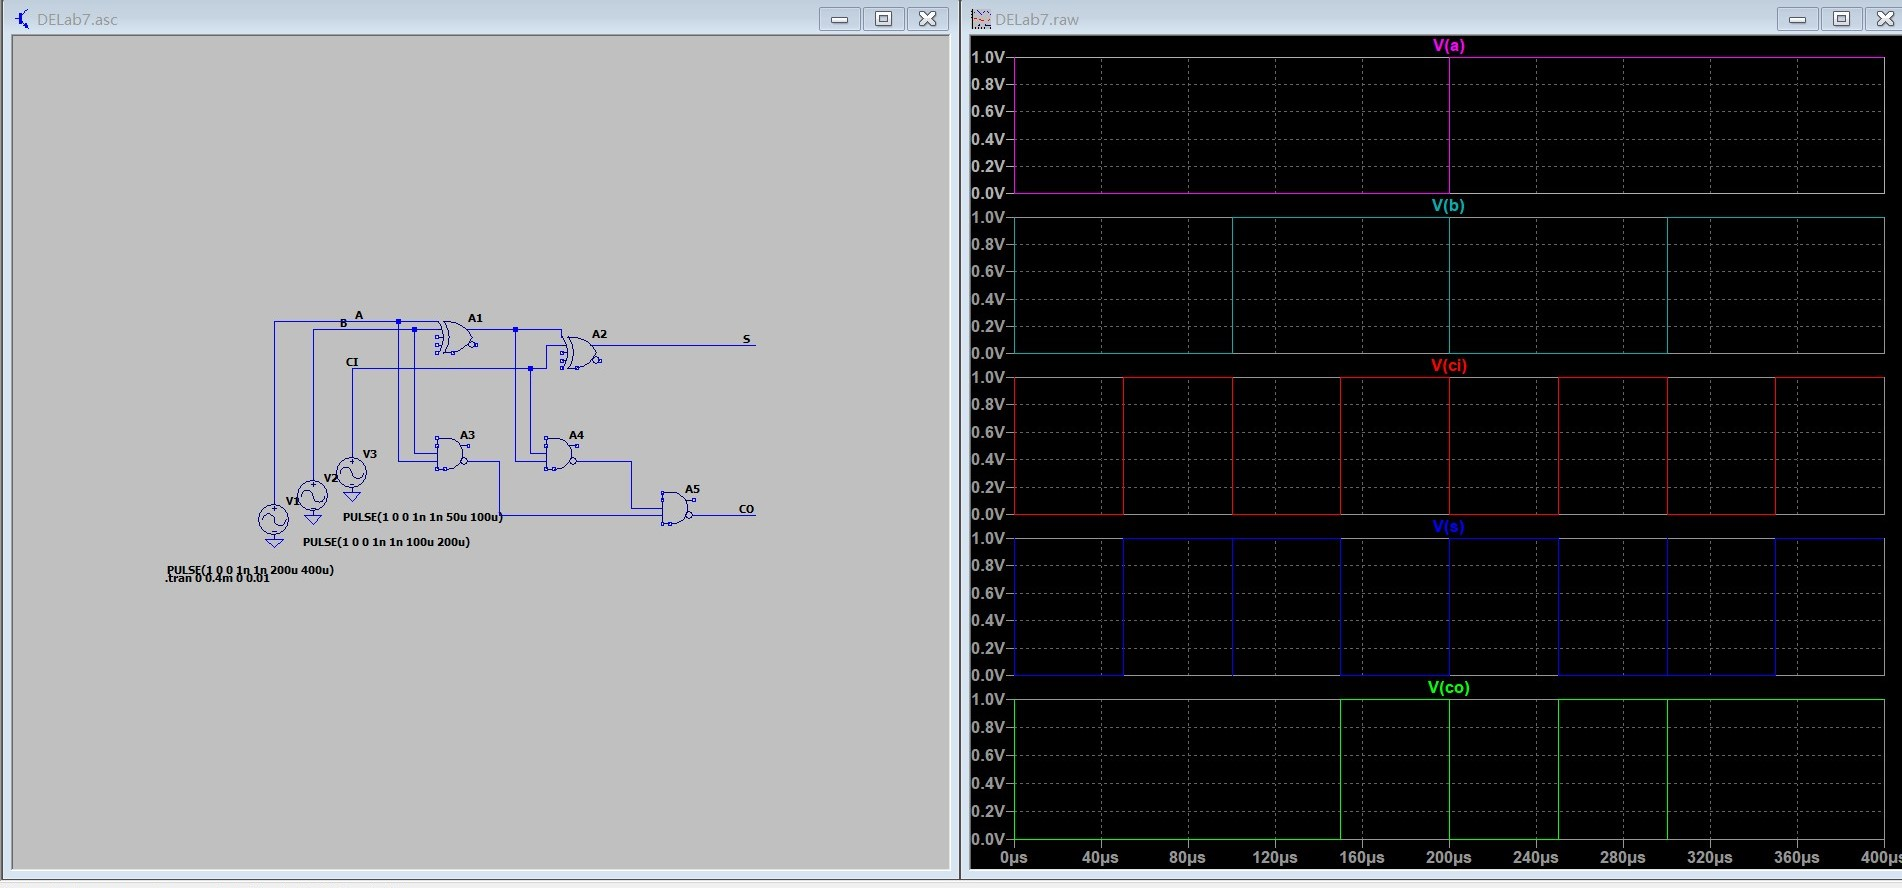
\includegraphics[width = 0.8\textwidth]{1-1仿真.jpg}
    \caption{1位二进制全加器-异或门,与非门}
\end{figure}

实际搭建电路,用二极管模拟输出的1/0,验证了电路的正确性。

\subsection*{2、用异或门和与门实现任务1(选做)}

如果仅使用异或门和与门来实现任务1,那么我们需要对$CO$的逻辑关系进行一些变形。

注意到$CO = (A \oplus B)CI + AB = (A \oplus B)CI \oplus AB$,之所以可以将或换成异或的原因是
$(A oplus B)CI$和$AB$不可能同时为1。

于是我们可以设计如下电路:

\begin{figure}[H]
    \centering
    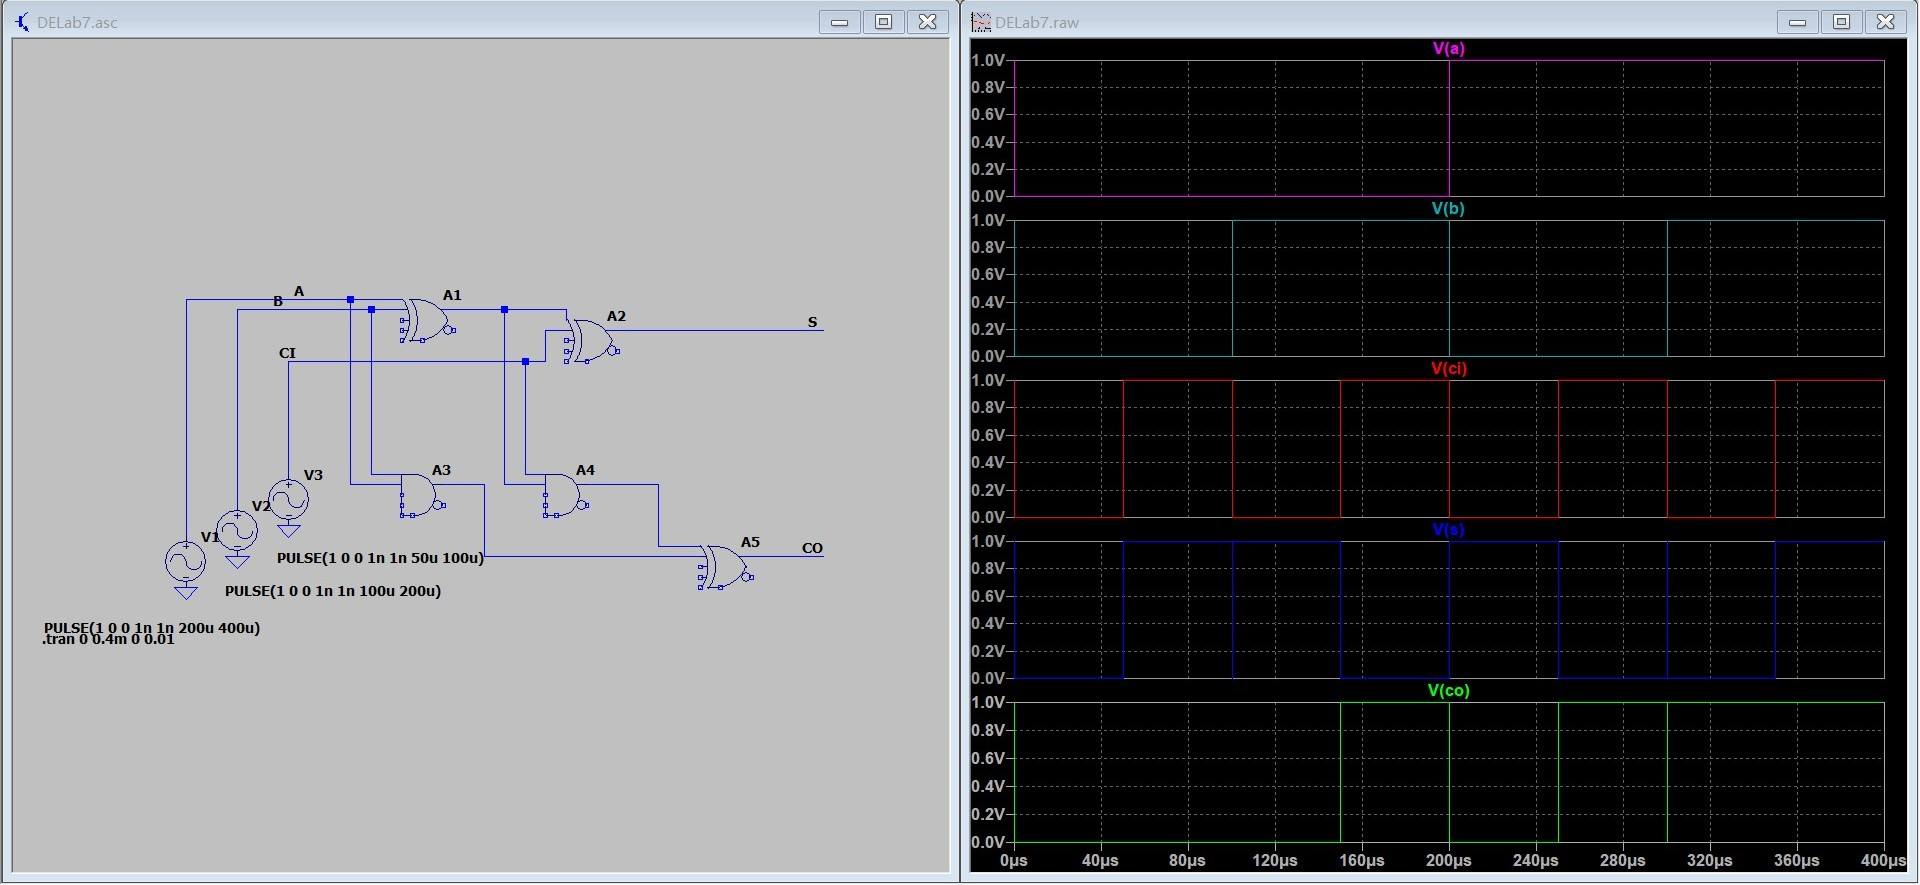
\includegraphics[width = 0.8\textwidth]{1-2仿真.jpg}
    \caption{1位二进制全加器-异或门,与门}
\end{figure}

仿真结果与预期相符,实际搭建电路,用二极管模拟输出的1/0,验证了电路的正确性。

实际电路图:
\begin{figure}[H]
    \centering
    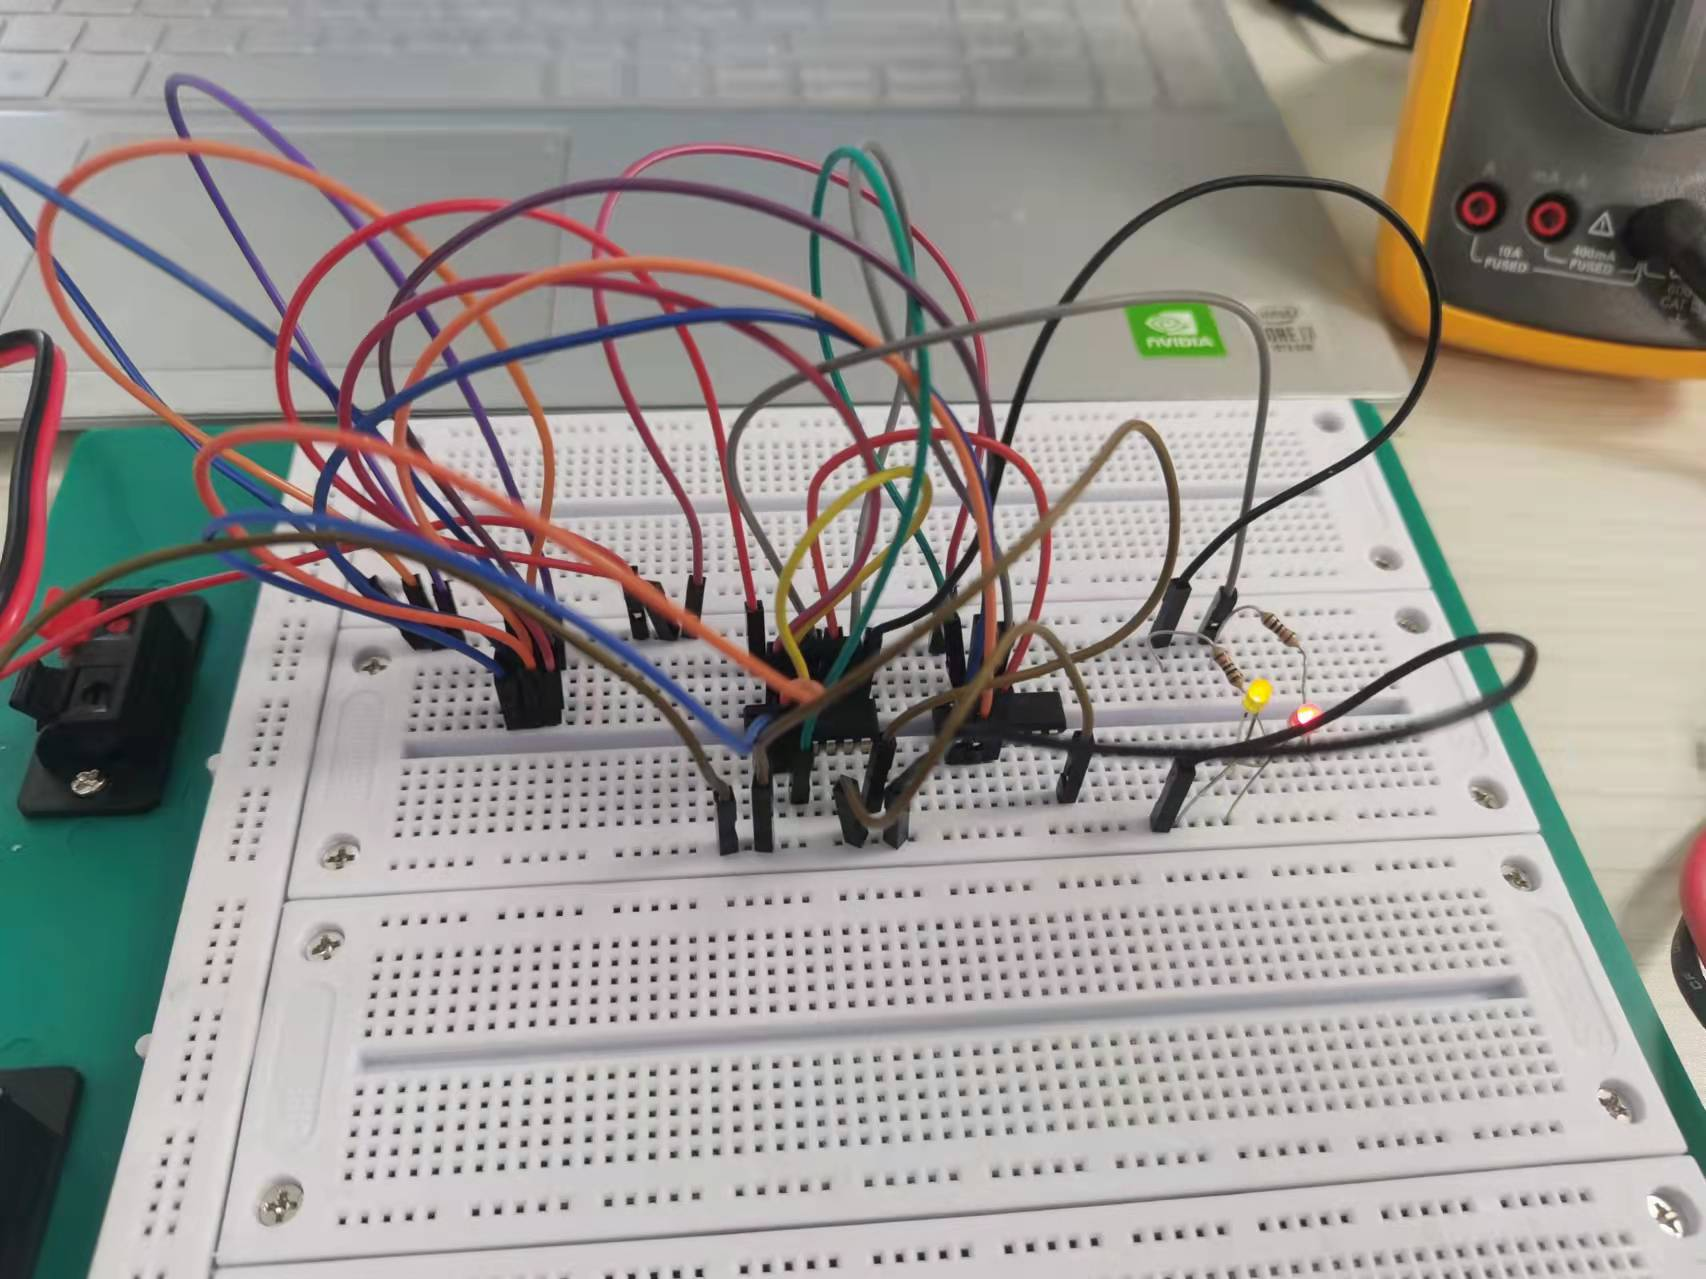
\includegraphics[width = 0.5\textwidth]{1-2-r-1.jpg}
    \caption{1位二进制全加器-异或门,与门实际电路图(1b+1b+1b=11b)}
\end{figure}

\begin{figure}[H]
    \centering
    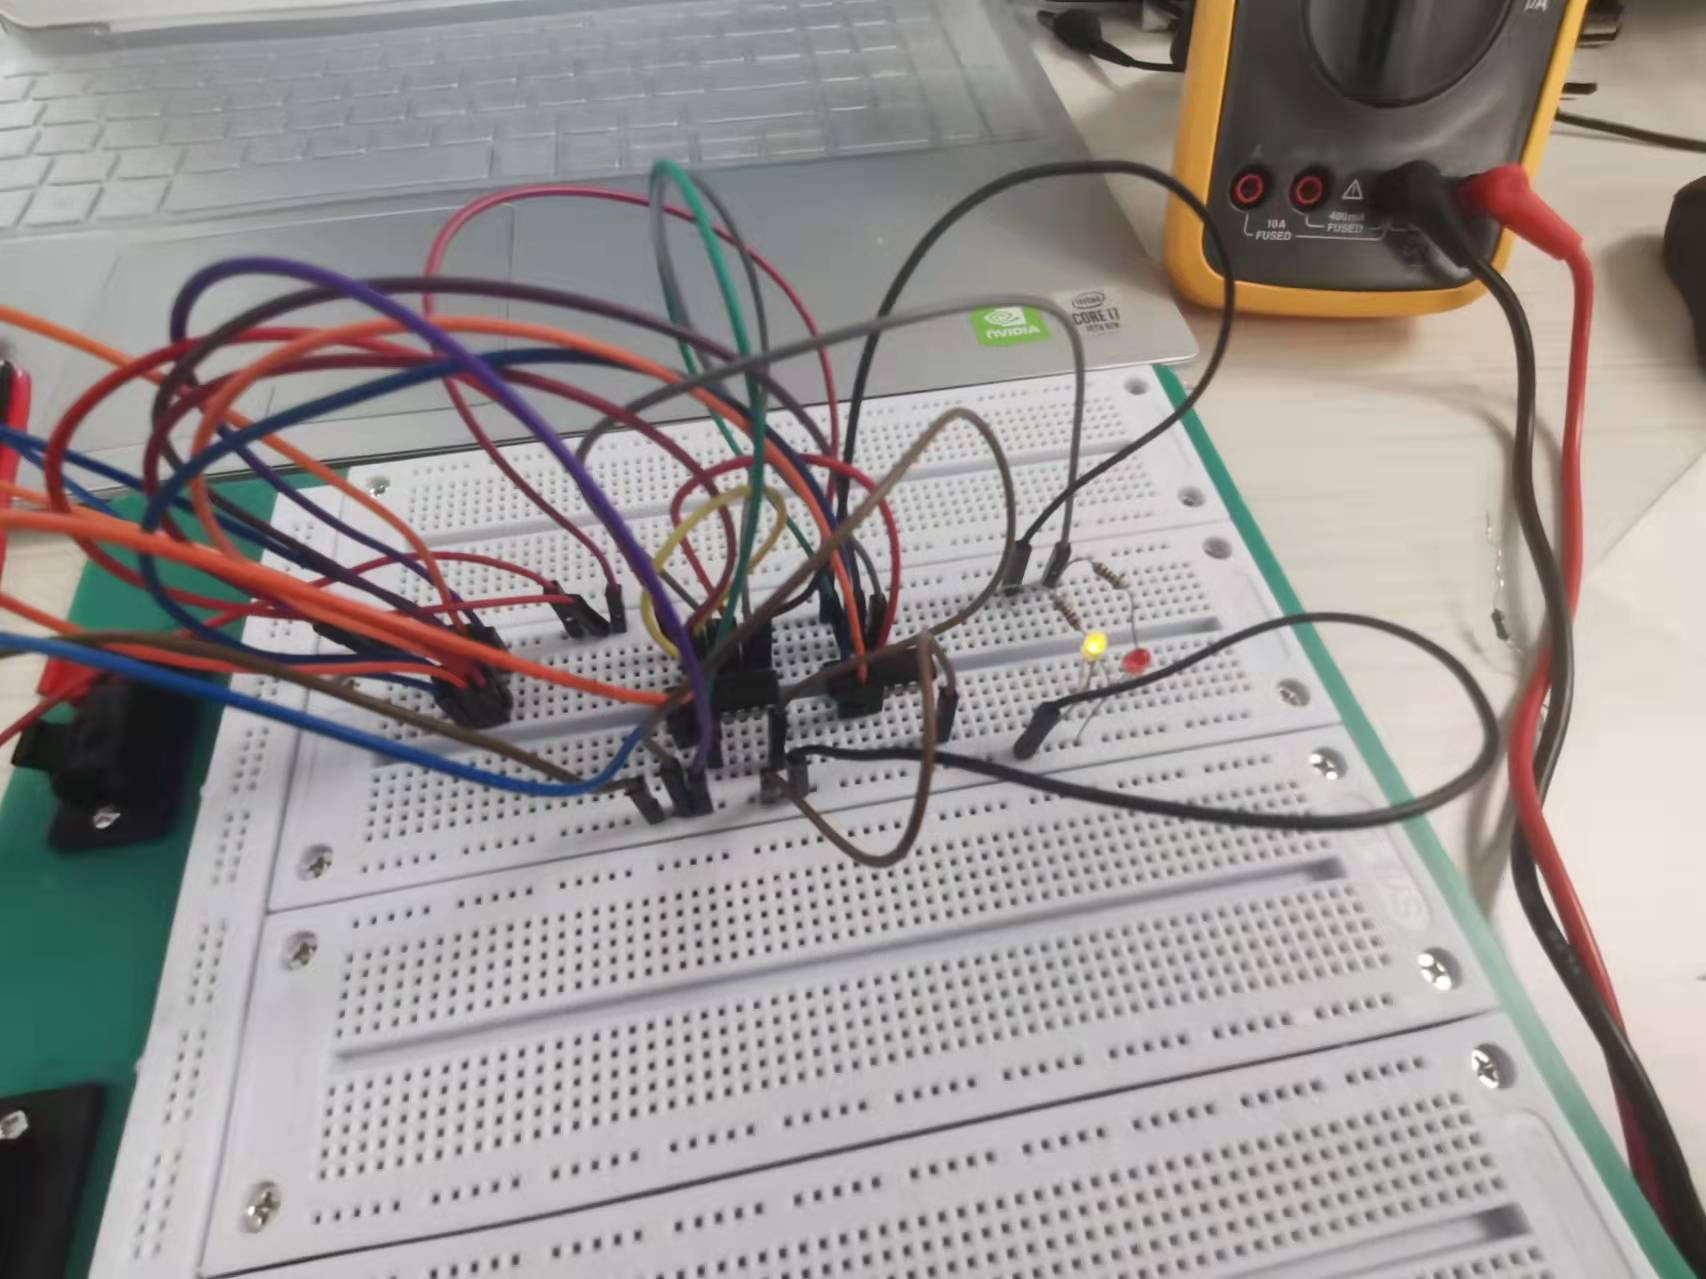
\includegraphics[width = 0.5\textwidth]{1-2-r-2.jpg}
    \caption{1位二进制全加器-异或门,与门实际电路图(1b+1b+0b=10b)}
\end{figure}
\noindent
备注:因为这部分选做是最后做的,上课还有一点时间,所以拍了照片,其余部分均已找祁硕老师验收。

\subsection*{3、用与上面实现方式不同的另一种电路完成任务1}

不同实现方式的本质是逻辑方式的替换,本部分我们将任务1中的与非门拆分成与门和非门,
而非门我们使用异或门与1相连实现。

逻辑变化式为
\begin{align*}
    CO &= \overline{ \overline{(A \oplus B)CI}\ \overline{AB} }\\
        &= (\overline{(A \oplus B)CI}\ \overline{AB}) \oplus 1
\end{align*}

仿真结果为:

\begin{figure}[H]
    \centering
    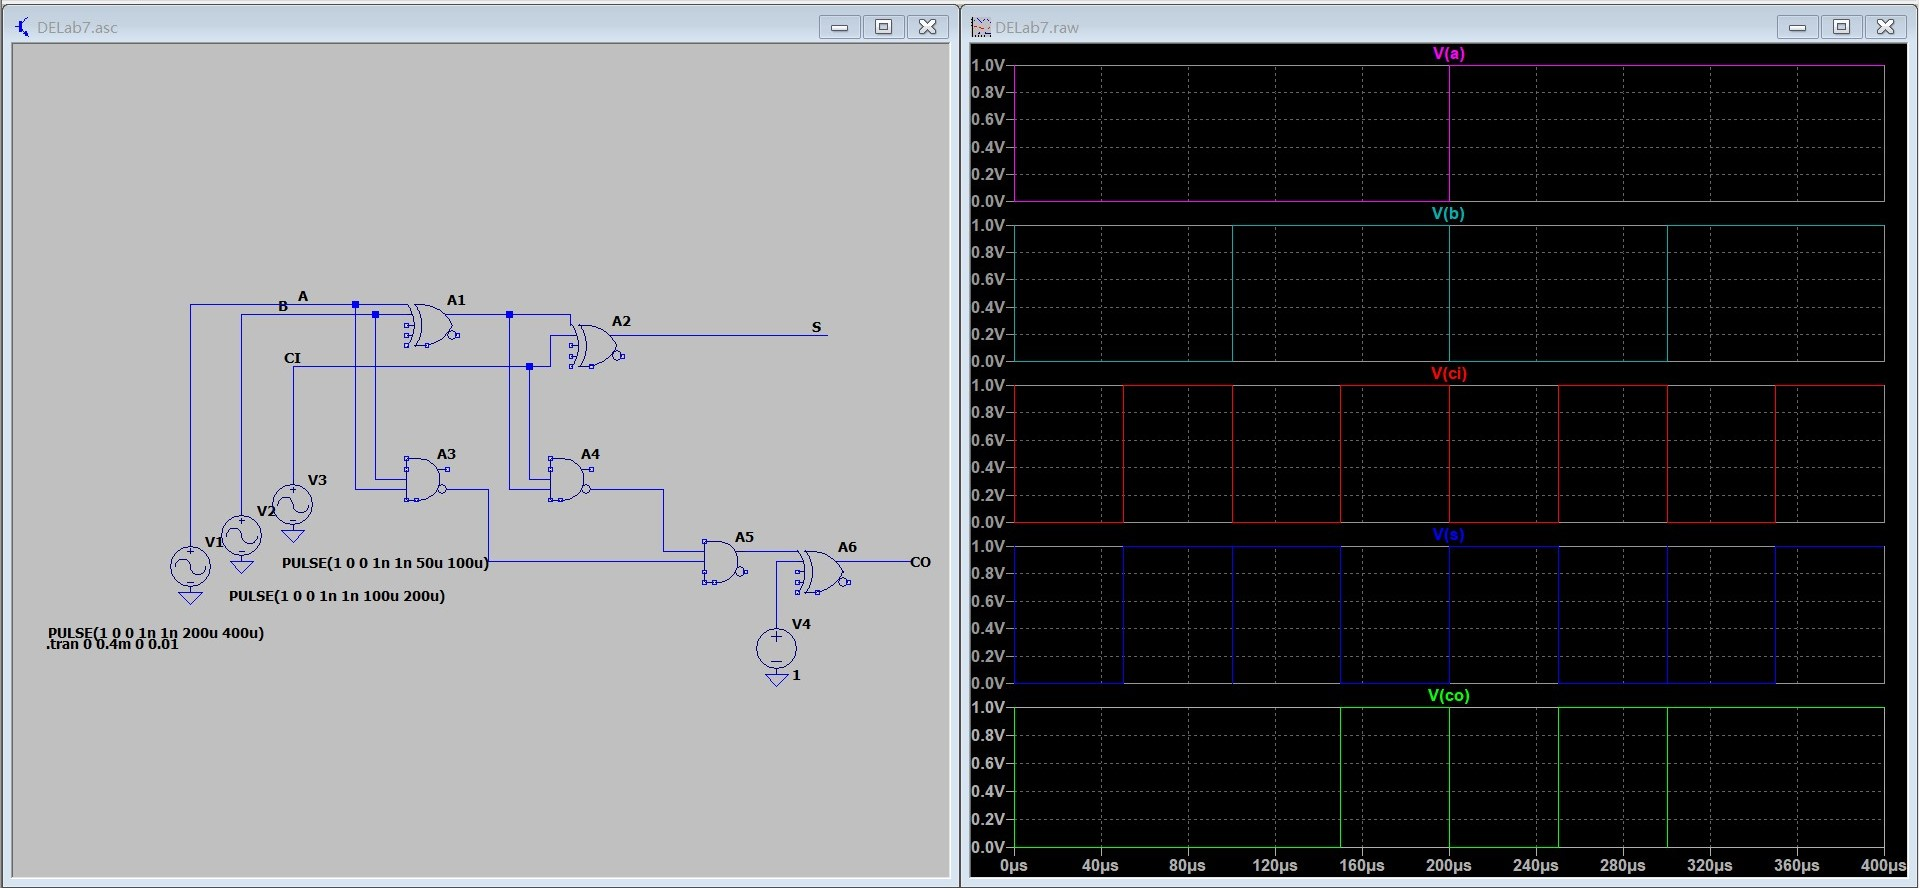
\includegraphics[width = 0.8\textwidth]{1-3仿真.jpg}
    \caption{1位二进制全加器-异或门,与门,与非门}
\end{figure}

仿真结果与预期相符,实际搭建电路,用二极管模拟输出的1/0,验证了电路的正确性。

\subsection*{4、设计4位全加器,画出电路图(不要求搭具体实现电路)}

在1位全加器的基础上,我们可以设计四位全加器。
我们先给1位全加器增加输入输出引脚,这里我们使用任务一的全加器:

\begin{figure}[H]
    \centering
    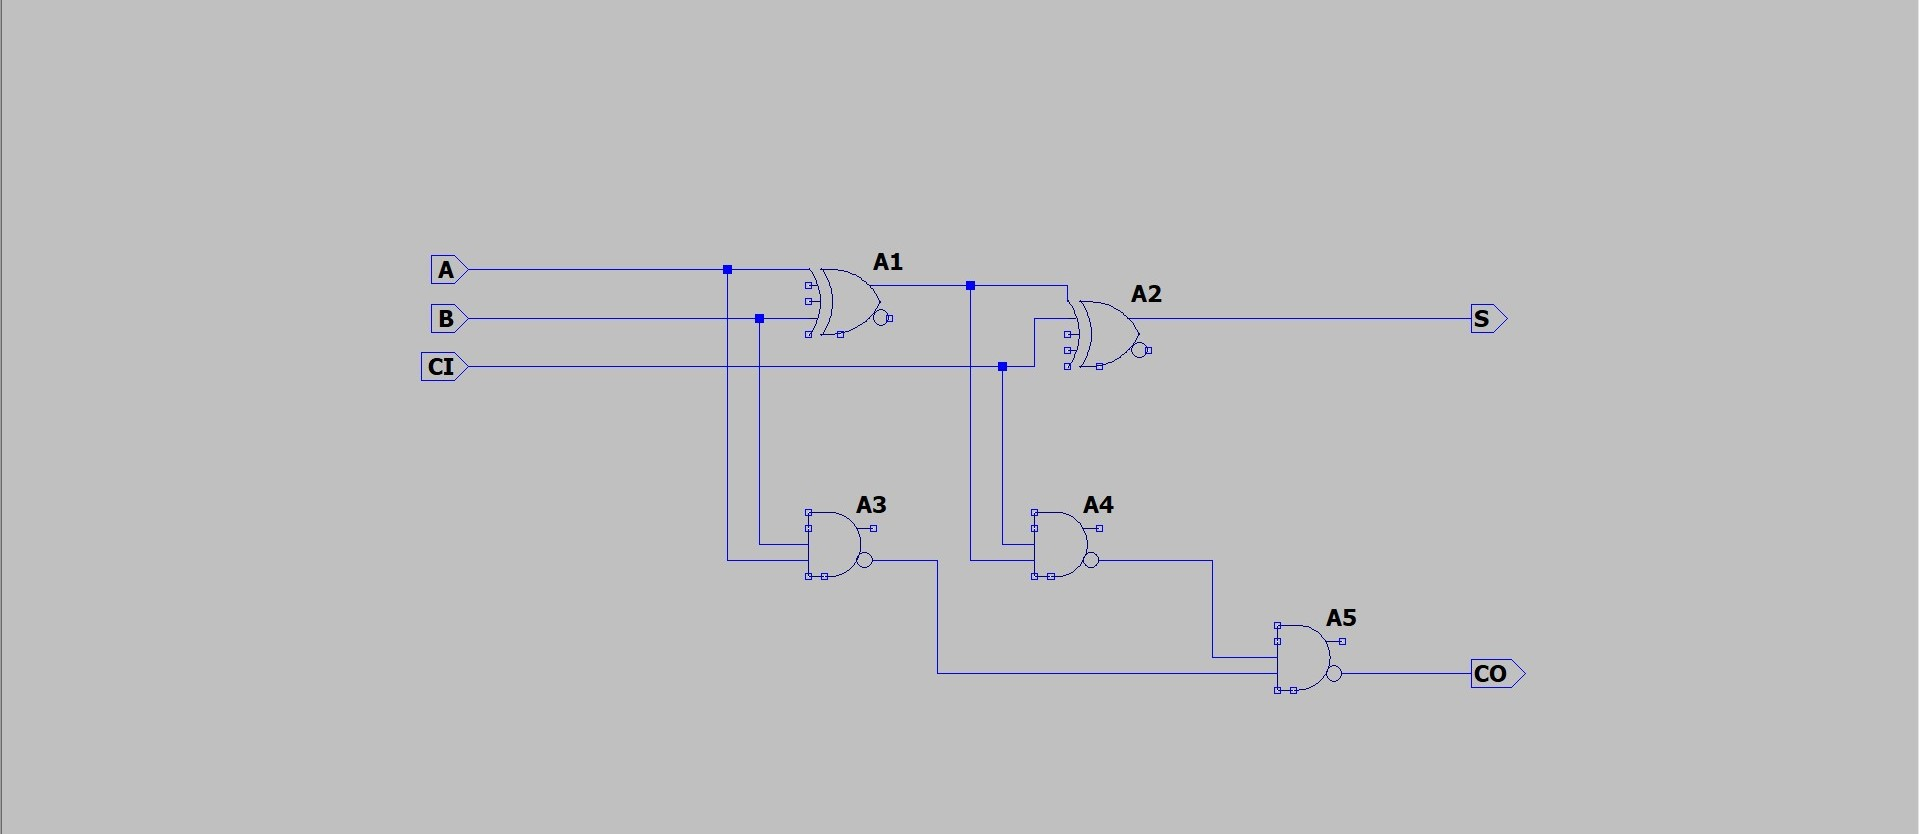
\includegraphics[width = 0.6\textwidth]{1位全加器.jpg}
    \caption{1位全加器}
\end{figure}

接下来我们通过create Symbol对1位全加器进行封装:

\begin{figure}[H]
    \centering
    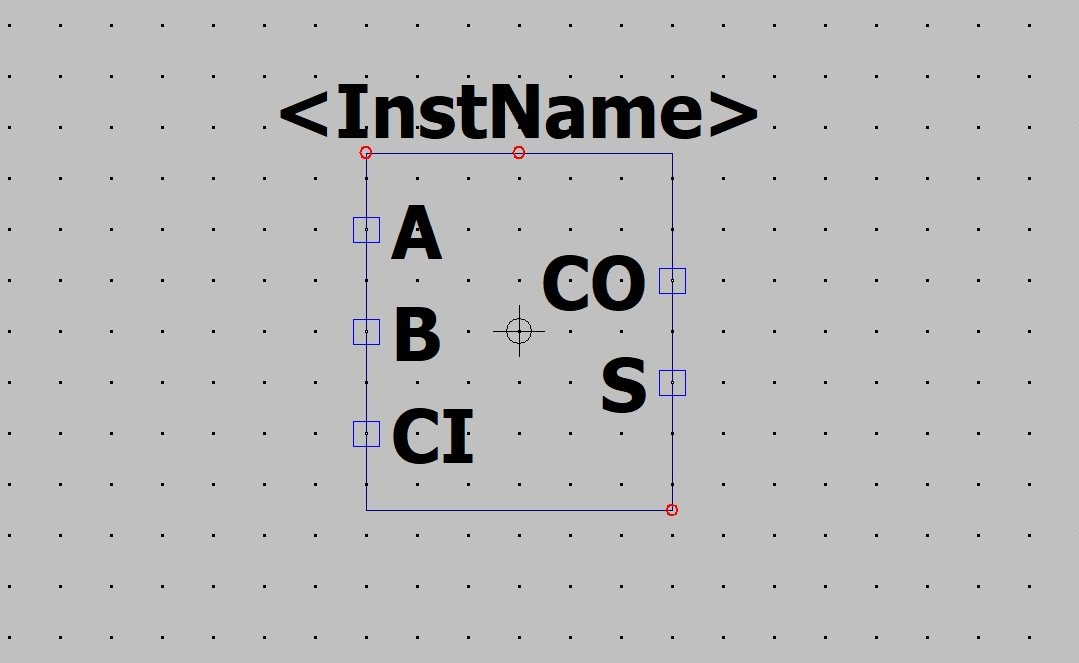
\includegraphics[width = 0.3\textwidth]{1位全加器封装.jpg}
    \caption{1位全加器封装}
\end{figure}

我们就可以根据1位全加器设计出最简单的4位串行全加器了,电路图如下:

\begin{figure}[H]
    \centering
    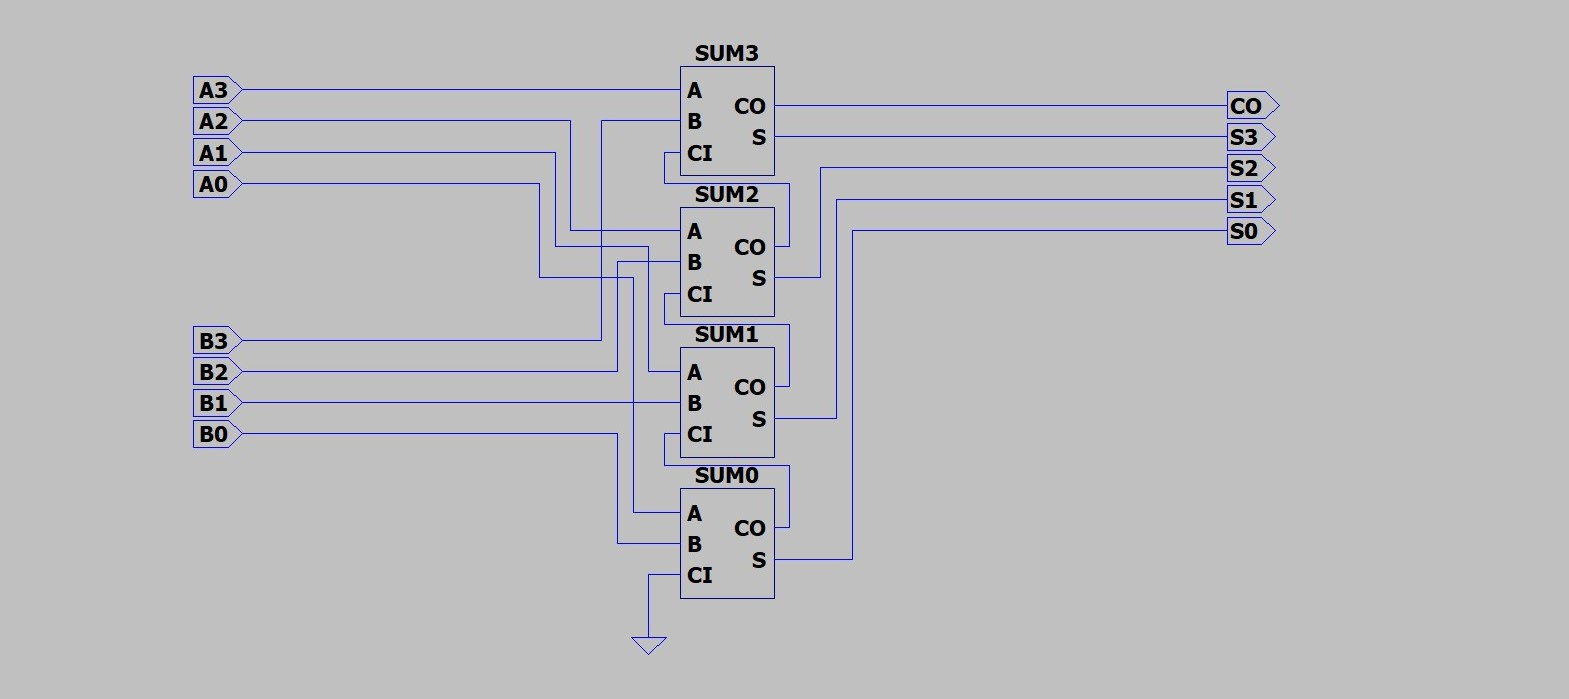
\includegraphics[width = 0.6\textwidth]{4位串行进位全加器.jpg}
    \caption{4位全加器}
\end{figure}

可以对4位全加器进行简单的验证,以下是其中一个验证结果:

\begin{figure}[H]
    \centering
    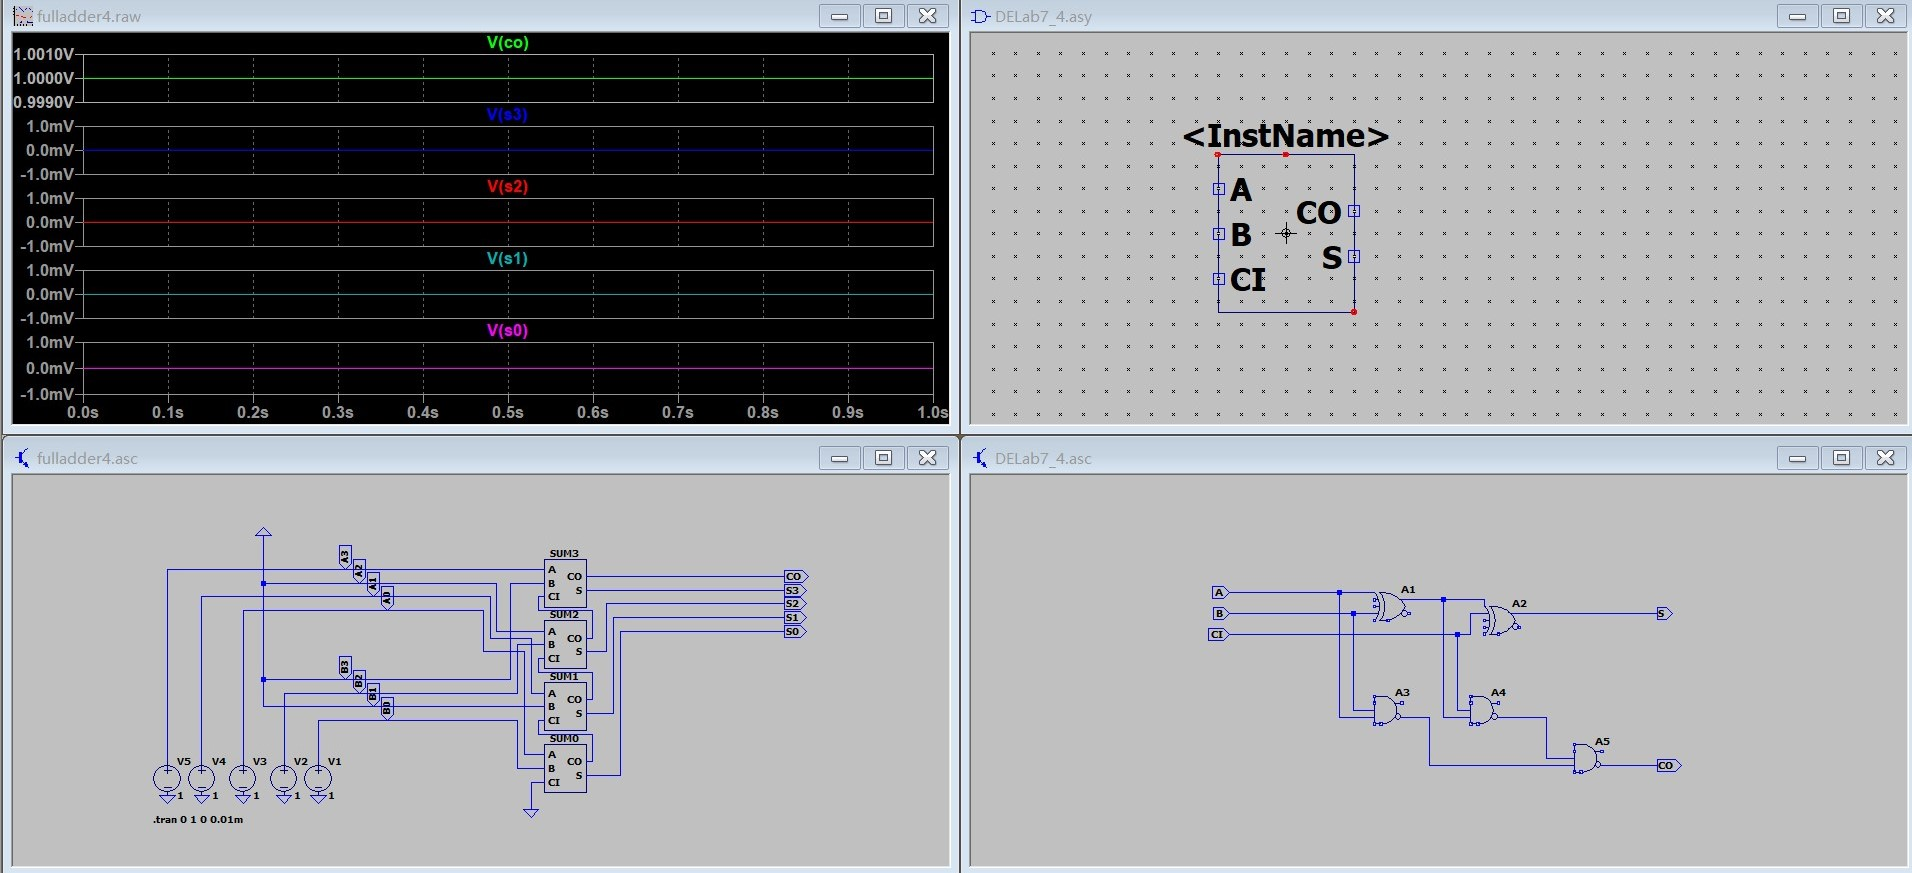
\includegraphics[width = 0.8\textwidth]{4位串行加法器仿真.jpg}
    \caption{4位全加器仿真验证(0101B + 1011B = 10000B)}
\end{figure}

仿真结果与预期相符合。

\end{document}